\begin{figure*}[h!]
\centering
\begin{adjustwidth}{-1em}{-1em}
\vspace*{-2ex}
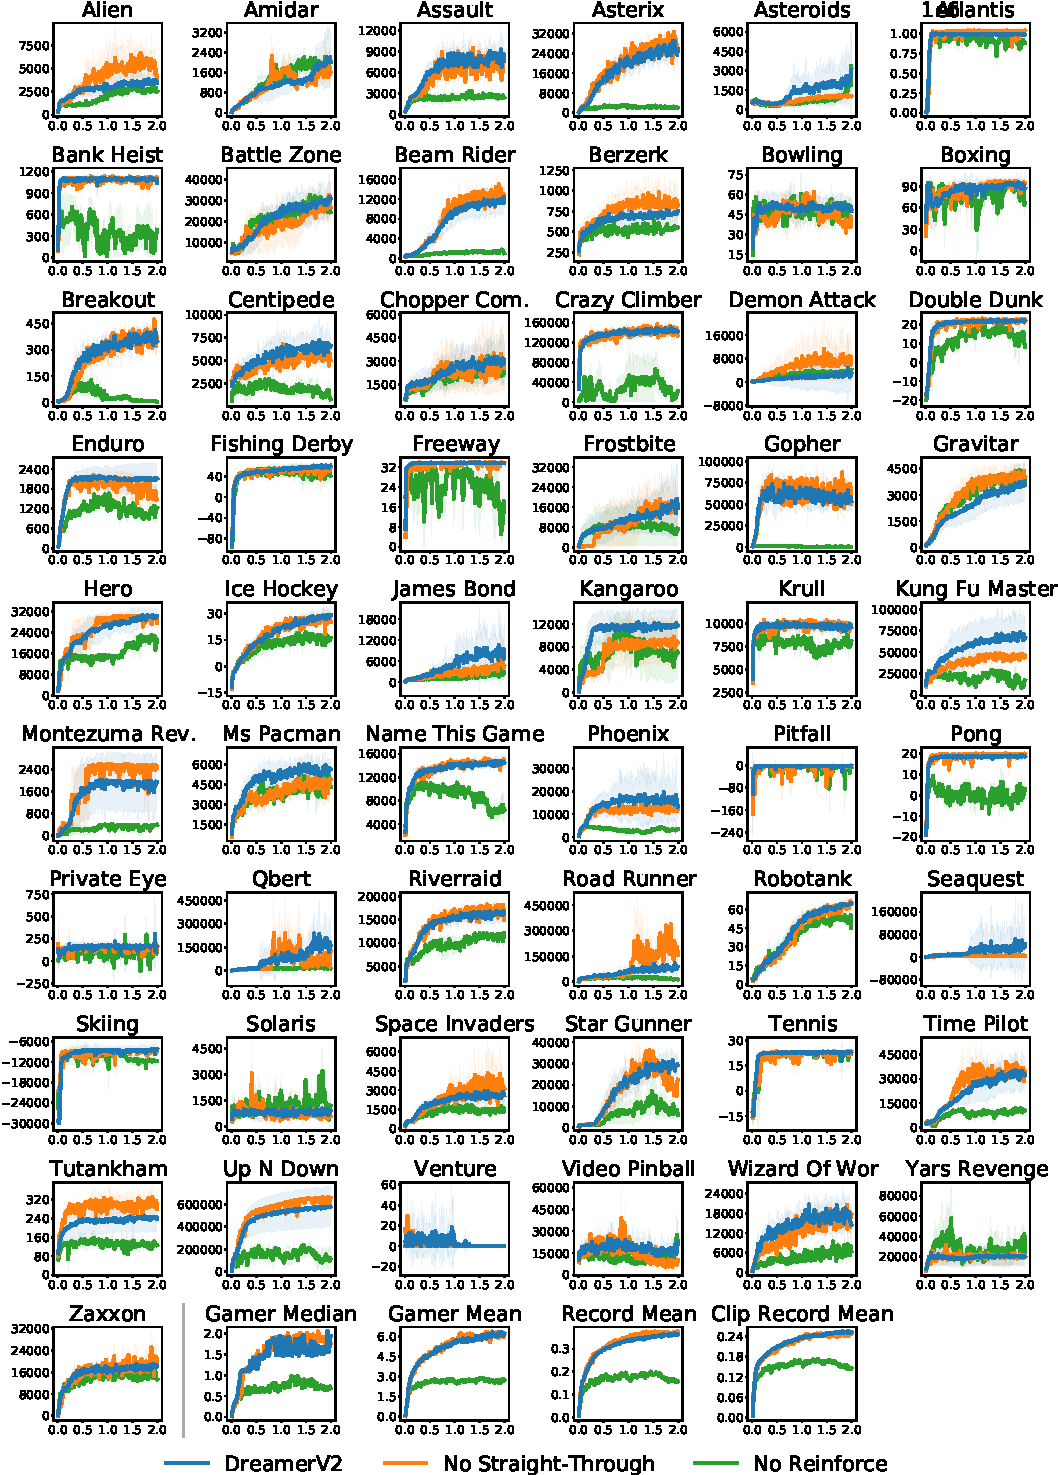
\includegraphics[width=\linewidth]{tasks-policy/tasks-policy}
\end{adjustwidth}
\caption{Comparison of leveraging Reinforce gradients, straight-through gradients, or both for training the actor. While Reinforce gradients are crucial, straight-through gradients are not important for most of the tasks. Nonetheless, combining both gradients yields substantial improvements on a small number of games, most notably on Seaquest. We conjecture that straight-through gradients have low variance and thus help the agent start learning, whereas Reinforce gradients are unbiased and help converging to a better solution.}
\label{fig:tasks-policy}
\vspace*{-3ex}
\end{figure*}
